\chapter{Results and Discussion}

\section{Qualitative Response Data}

Written user responses showed that for the features that did work, it was an incredibly positive experience for the user in the moment. Many users reported within the survey that they were not even going to attempt to look at the university’s current system as that simply was too much work and preferred by far to use the web application demo provided. It was also noted that of the user responses, there was a question that asked for any technical difficulties or negative experiences and over half of the users either gave no response or N/A.

\begin{table}[H]
\centering
\begin{tabularx}{\linewidth}{X|X}
\toprule
\textbf{Advantages of Microsoft Document} & \textbf{Demo Feedback and Additional Features}\\
\midrule
No & Seems to work well, would like better error messages when creating an account with a password that does not meet requirements.\\
The ability for a medical professional to give supporting evidence of your circumstances & Received a "Form service failed! Is it maybe down?" error for the forms I tried to submit. Not sure if that is intentional. Otherwise, everything ran well.\\
You can see everything you need to fill out ahead of time all at once & N/A\\
I enjoyed it & No\\
I was unable to access the Microsoft document & Confirmation of which boxes were not filled out\\
N/A & I was genuinely confused as to how to use the system, as it seemed as though it should use my own university login details given how professional it looks.\\
Would be harder to spam the department with joke forms & The form will not tell you if bad data is input but will not submit the form (i.e., name and reg no. not matching the account or invalid date).\\
N/A & Department details: "I was able to sign up with a 10-digit registration code when I'm supposed to only be able to submit a 9-digit number. When filling out a form (and using a 9-digit reg number), I added 5 modules, some of which were added after attempting to submit, but every time, it refused to submit the form. It worked once I refreshed the page to try again."\\
No, I hate the University system & No, the demo worked as expected.\\
No, the online form is WAY better (I couldn't even find the extenuating circumstances form when I tried and then just gave up lol) & I wanted to only submit one form (or for one module really), but it wouldn't let me go to the next page without filling out another one (might be my bad but still).\\
\bottomrule
\end{tabularx}
\caption{User Feedback and Suggestions}
\label{tab:user_feedback_table}
\end{table}

As seen in Table \ref{tab:user_feedback_table}, there were a varity of user experience ranging from purely positive to only a few issues that happened with early setup of the demo. Some of the first responses were used in section 5.2 to assist with quick patches for future users.
\newline
\newline
While this demo is an attempt to serve those in need and all responses were taken to further improve the research on developing an application to serve all, this level of high responsiveness to only positive feedback was a good sign that the demo was beginning to solve the root problem. It was also noted from one user that, “I was genuinely confused as to how to use the system, as it seemed as though it should use my own university login details given how professional it looks”. This feedback in particular was very nice to see from a developer standpoint and did show that the parts of the UI that were polished felt extremely user friendly. The downside to comments like these however, is that it does not provide much insight into furthering the application’s ability to assist but rather is just a compliment on system artwork.
 
\section{Static File Serving}

With the request to upload files being an incredibly high demand feature, this would certainly be the logical next step in implementing to solve user issues with proof for their extenuating circumstances. One of the reasons this was not implemented in the demo was there was a fear of viewing some of the uploaded images that users could post. After reading through some of the sample uses of the database, users did have the ability to submit data that was not actually related to the extenuating circumstance form at all, but rather were posting dummy data for the sake of seeing how the system would respond. For a demo setting this is perfectly acceptable however one of the easy to implement features down the line this presents is a word checker for inappropriate behaviour within the school system.
\newline
\newline
Without the ability to carefully scan images with the current time constraints of demo development, this made it such that the development team did not desire to look at sample pdfs and images provided by the users. This would also present a whole set of new routing protocols that would have to be set up by Nginx, as static files provide routes of sending injection attacks back to the server and a correct routing protocol would need to be added. Django provides explicit instructions that only in development servers can static media be sent back to a user, and it is recommended that a WSGI server be used as a mediator between the frontend client and the backend server due to these security risks.
\newline
\newline
The fortunate part of this project is that given the structure, it is incredibly easy to implement an upload feature down the line for users to include as much media as they desire within the form. Utilising the power of React’s component based system, all that is needed is a new component to be added to the form for media attachment and posting to the backend at a newly created route. This would solve the high user demand for being able to attach media to the form and only creates the difficulty then of serving this data back to the user or an administrator.

\begin{figure}[H]
\centering
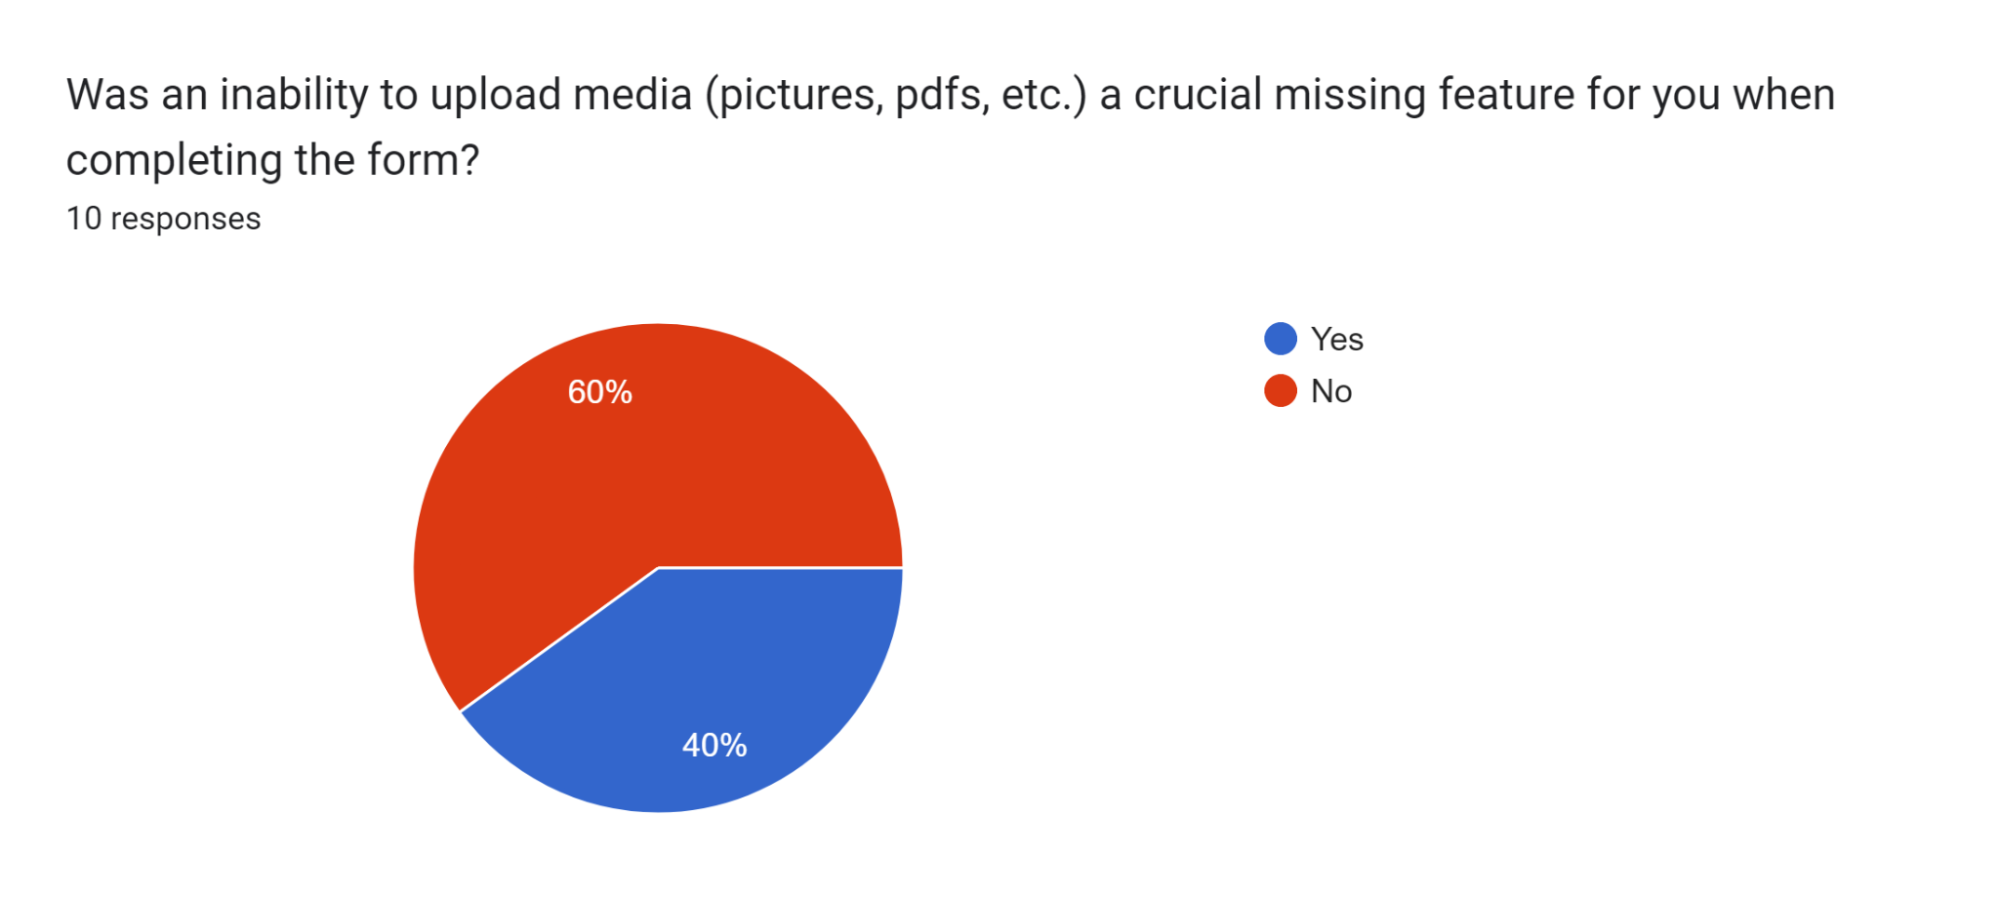
\includegraphics[width=15cm]{myReport/images/static_upload.png}
\caption{User demand for being able to upload images}
\label{fig:static_upload}
\end{figure}

As seen from Figure \ref{fig:static_upload}, there was an unsuprising demand for being able to upload images or PDFs, however this was not a complete set of users. This would be the next priority for development given how many users did request this feature though.
 
\section{Scalability}

One of the issues quickly learned was working with growing to more users. While running the demo on one single core computer is fine for a demo, there is the potential issue if two or 3 users try to access the system that responses become significantly slowed down. A variety of factors contribute to this, with the first being that the database is a single system running without a cluster.
\newline
\newline
This makes it so that each time a read or write is done, it cannot be done concurrently and has to wait for the previous operation to be completed. This means that if many user accounts are logged in at the same time trying to complete operations such as submitting forms, this drastically decreases performance. One of the first solutions researched and mentioned in section 2.6 is the use of a caching layer or even the implementation of a whole caching database such as Redis. This would provide the ability for the server to grab data from RAM rather than read and write to disk. This demo in particular was deployed and running on a hard drive rather than a solid state drive or even an NVME ssd, which further amplified the time it takes to complete certain queries.
\newline
\newline
One of the quickest ways to complete a quick patch to this issue without complete migration or structural changes is to improve the way in which queries are made. With hindsight after having developed the project, it is far easier to pull more entries out of a table and leverage using CASE rather than UPDATE requests to the database. This makes it so that when an instruction is executed, the case can do a batch update rather than an iterative update using the WHERE clause. The difficulties in creating these types of operations was not realised when development first started but would create the opportunity to vastly boost performance, especially as the database grows in size and complexity of tables.
\newline
\newline
Another option moving forward would be to develop microservices and begin to split off certain functionality to provide constant uptime no matter what real world events affect the server. Should a downtime occur, it requires a reboot of the system automatically or even manual human intervention to get the entire frontend and backend back running. For the flipside, there should always be the ability for a user to at least get to the homepage, if not login at minimum. This cannot be done with a monolithic project as structured in the current demo, but as shown in section 2.1 would provide the constant understanding to users that something has gone wrong internally and give them a message to come back later instead. This need is further compounded by the original issue that this demo is trying to serve those in need and are facing extenuating circumstances affecting their studies. Having a system that helps guide a user from start to finish is critical as shown in the survey and day one patch and should not ever go down in mass scale.